\section{Experiments}
\label{sec:experiments}

We present the experimental protocol used to evaluate \textbf{instruction-driven, runtime-switchable alignment}.
The central question is not whether a model can follow instructions in the usual sense, but whether it can \textbf{counterfactually switch alignment posture}:
\textbf{holding the user prompt fixed} while varying \textbf{only} the alignment instruction (policy contract).
We therefore design experiments that separate (i) \textbf{base capability} from (ii) \textbf{instruction sensitivity}, and that compare SwiPO against both \textbf{offline preference} and \textbf{online RL} baselines under a consistent training stack.

\vspace{-0.2em}
\paragraph{\textbf{Overview.}}
We train Llama-3.1-8B with LoRA adapters through a staged pipeline (Base $\rightarrow$ SFT $\rightarrow$ DPO $\rightarrow$ SwiPO), and construct matched \textbf{NoInstruct} and \textbf{Instruct} variants for each method.
NoInstruct uses standard prompts; Instruct prepends an explicit \textbf{behavioral contract} instruction (epistemic stance, refusal boundary, verbosity) to the same user request.
The primary readout is \textbf{instruction sensitivity} $\Delta$ (Instruct $-$ NoInstruct), which directly measures how much a method exposes a \textbf{controllable alignment channel} rather than a static policy baked into weights.

% -----------------------------------------------------------------------------
\vspace{-1mm}
\subsection{Training Pipeline}
\label{sec:appendix_training_pipeline_exp}

Following the staged approach in Section~\ref{sec:cita_framework}, we train on PKU-SafeRLHF~\cite{ji2024pku,bai2022training} using NVIDIA A100 GPUs and LoRA~\cite{hu2022lora} adapters.
Offline preference methods (SFT/DPO/SwiPO) run on A100-40GB, while online methods (PPO/GRPO) require A100-80GB due to on-policy generation and reward evaluation overhead.
The pipeline is designed to isolate a practical deployment claim:
\textbf{\emph{instruction-driven alignment is most meaningful when applied on top of an already-aligned policy}}, since the instruction channel should modulate a safe neighborhood rather than repair a fundamentally unsafe base.

\vspace{-0.2em}
\paragraph{\textbf{Stages.}}
Training proceeds through four stages:

\begin{enumerate}[leftmargin=*,itemsep=1pt]
    \item \textbf{Base}: Llama-3.1-8B~\cite{dubey2024llama} pretrained weights.
    \item \textbf{SFT}: Supervised fine-tuning on PKU \emph{chosen} responses to establish a strong instruction-following and safety baseline.
    \item \textbf{DPO}: Offline preference optimization on PKU preference pairs to strengthen alignment via direct preference shaping.
    \item \textbf{SwiPO}: Instruction-conditioned preference learning with an explicit stability anchor (trust-region style) to preserve a \textbf{switchable policy family} rather than collapsing to one dominant stance.
\end{enumerate}

\vspace{-0.2em}
\paragraph{\textbf{Why this ordering matters.}}
We emphasize the ordering because instruction-driven alignment is not intended as a substitute for base alignment.
Instead, it adds a \textbf{runtime control interface} over an already aligned manifold:
SwiPO learns to \textbf{navigate} between nearby regimes (e.g., strict vs.\ permissive safety; honest vs.\ confident epistemics; concise vs.\ detailed verbosity) without requiring separate checkpoints.

% -----------------------------------------------------------------------------
\vspace{-1mm}
\subsection{Model Variants}
\label{sec:model_variants}

We train 10 variants spanning 5 methods (SFT, PPO, GRPO, DPO, SwiPO) $\times$ 2 instruction settings (NoInstruct, Instruct).
This factorial design supports two comparisons:
\textbf{(i) within-method switching} (NoInstruct vs.\ Instruct) to quantify instruction sensitivity, and
\textbf{(ii) cross-method switching} to compare how different optimization paradigms expose (or suppress) an alignment instruction channel.

\begin{table*}[ht!]
\centering
\normalsize
\renewcommand{\arraystretch}{1.2}
\begin{tabular}{@{}lll@{}}
\toprule
\textbf{Model} & \textbf{Training Path} & \textbf{Instruction} \\
\midrule
SFT\_NI & Base$\rightarrow$SFT & No \\
\hline
SFT\_I & Base$\rightarrow$SFT & Yes \\
\hline
PPO\_NI & Base$\rightarrow$SFT$\rightarrow$PPO & No \\
\hline
PPO\_I & Base$\rightarrow$SFT$\rightarrow$PPO & Yes \\
\hline
GRPO\_NI & Base$\rightarrow$SFT$\rightarrow$GRPO & No \\
\hline
GRPO\_I & Base$\rightarrow$SFT$\rightarrow$GRPO & Yes \\
\hline
DPO\_NI & Base$\rightarrow$SFT$\rightarrow$DPO & No \\
\hline
DPO\_I & Base$\rightarrow$SFT$\rightarrow$DPO & Yes \\
\hline
SwiPO\_NI & Base$\rightarrow$SFT$\rightarrow$DPO$\rightarrow$SwiPO & No \\
\hline
SwiPO\_I & Base$\rightarrow$SFT$\rightarrow$DPO$\rightarrow$SwiPO & Yes \\
\bottomrule
\end{tabular}
\caption{\textbf{Model variants.} NI = NoInstruct (standard prompts), I = Instruct (behavioral contract prepended). PPO/GRPO/DPO branch from SFT; SwiPO stacks on DPO to learn instruction-conditioned switching under stability constraints.}
\label{tab:model_variants}
\vspace{-4mm}
\end{table*}

\vspace{-0.2em}
\paragraph{\textbf{Comparison design (what $\Delta$ means).}}
For each method, we compute instruction sensitivity as
\[
\Delta \;=\; \text{Score}(\text{Instruct}) \;-\; \text{Score}(\text{NoInstruct}).
\]
A large positive $\Delta$ indicates that the method exposes a \textbf{functional policy control channel}:
the alignment instruction changes behavior in the intended direction under an unchanged user request.
A near-zero $\Delta$ indicates \textbf{static alignment}: the method may be aligned, but the instruction channel is largely ignored.

% -----------------------------------------------------------------------------
\vspace{-1mm}
\subsection{Hyperparameter Optimization}
\label{sec:hyperparams_appendix}

We tune SwiPO's hyperparameters using Optuna~\cite{akiba2019optuna} with the TPE (Tree-structured Parzen Estimator) sampler, 13 completed trials per variant.
TPE is a Bayesian optimization strategy that models promising vs.\ unpromising configurations and proposes new trials by maximizing expected improvement under those density models.
The search maximizes three training-run objectives, final reward margin, preference accuracy, and negative validation loss (\texttt{src/train/cita\_optuna.py}); no evaluation suite enters it, so instruction sensitivity was not tuned for.

\vspace{-0.2em}
\paragraph{\textbf{Instruct training diverged at the NoInstruct learning rate.}}
SwiPO\_Instruct's selected learning rate ($5.4\times10^{-6}$) is 21\% below SwiPO\_NoInstruct's ($6.8\times10^{-6}$). An Instruct run at $6.83\times10^{-6}$ diverged, so the Instruct search range was capped below it; we did not test why.

\begin{table*}[ht!]
\centering
\normalsize
\setlength{\tabcolsep}{6pt}
\renewcommand{\arraystretch}{1.2}
\begin{tabular}{@{}lcc@{}}
\toprule
\textbf{Hyperparameter} & \textbf{NoInstruct (T5)} & \textbf{Instruct (T7)} \\
\midrule
Learning rate & 6.83e-6 & 5.41e-6 \\ \hline
$\lambda_{\text{KL}}$ & 0.00052 & 0.00023 \\ \hline
$\beta$ (DPO temp.) & 0.119 & 0.107 \\ \hline
Weight decay & 0.0091 & 0.0109 \\ \hline
Warmup ratio & 7.5\% & 10.0\% \\
\midrule
Final margin & 6.95 & 7.52 \\ \hline
Accuracy & 89.5\% & 89.0\% \\
\bottomrule
\end{tabular}
\caption{\textbf{Best hyperparameters from Optuna search.} T5/T7 denote the best trial IDs for NoInstruct and Instruct runs, respectively. The Instruct variant prefers a lower LR and a smaller $\lambda_{\text{KL}}$, while achieving a higher final reward margin at comparable accuracy.}
\label{tab:hyperparams_exp}
\vspace{-4mm}
\end{table*}

\vspace{-0.2em}
\paragraph{\textbf{Interpretation.}}
Two tuning patterns recur across trials.
\textbf{First,} $\beta$ exhibits a narrow ``Goldilocks'' band: too low weakens preference separation, too high inflates margins but can reduce instruction sensitivity by over-hardening a single stance.
\textbf{Second,} $\lambda_{\text{KL}}$ trades off \textbf{switchability vs.\ rigidity}: too small risks regime collapse, too large prevents meaningful motion between instruction regimes.

% -----------------------------------------------------------------------------
\vspace{-1mm}
\subsection{Training Dynamics}
\label{sec:appendix_training_dynamics}

We analyze training curves to understand how SwiPO differs from DPO in optimization behavior.
Additional plots (eval loss, SFT loss, token accuracy) are included in Appendix~\ref{sec:appendix_training_curves}.
We emphasize one operational point:
\textbf{accuracy alone is insufficient}.
High preference accuracy can coexist with poor switching if the model collapses into a single dominant posture.
We therefore track both \textbf{reward accuracy} and \textbf{reward margin}.

\begin{figure*}[ht!]
\centering
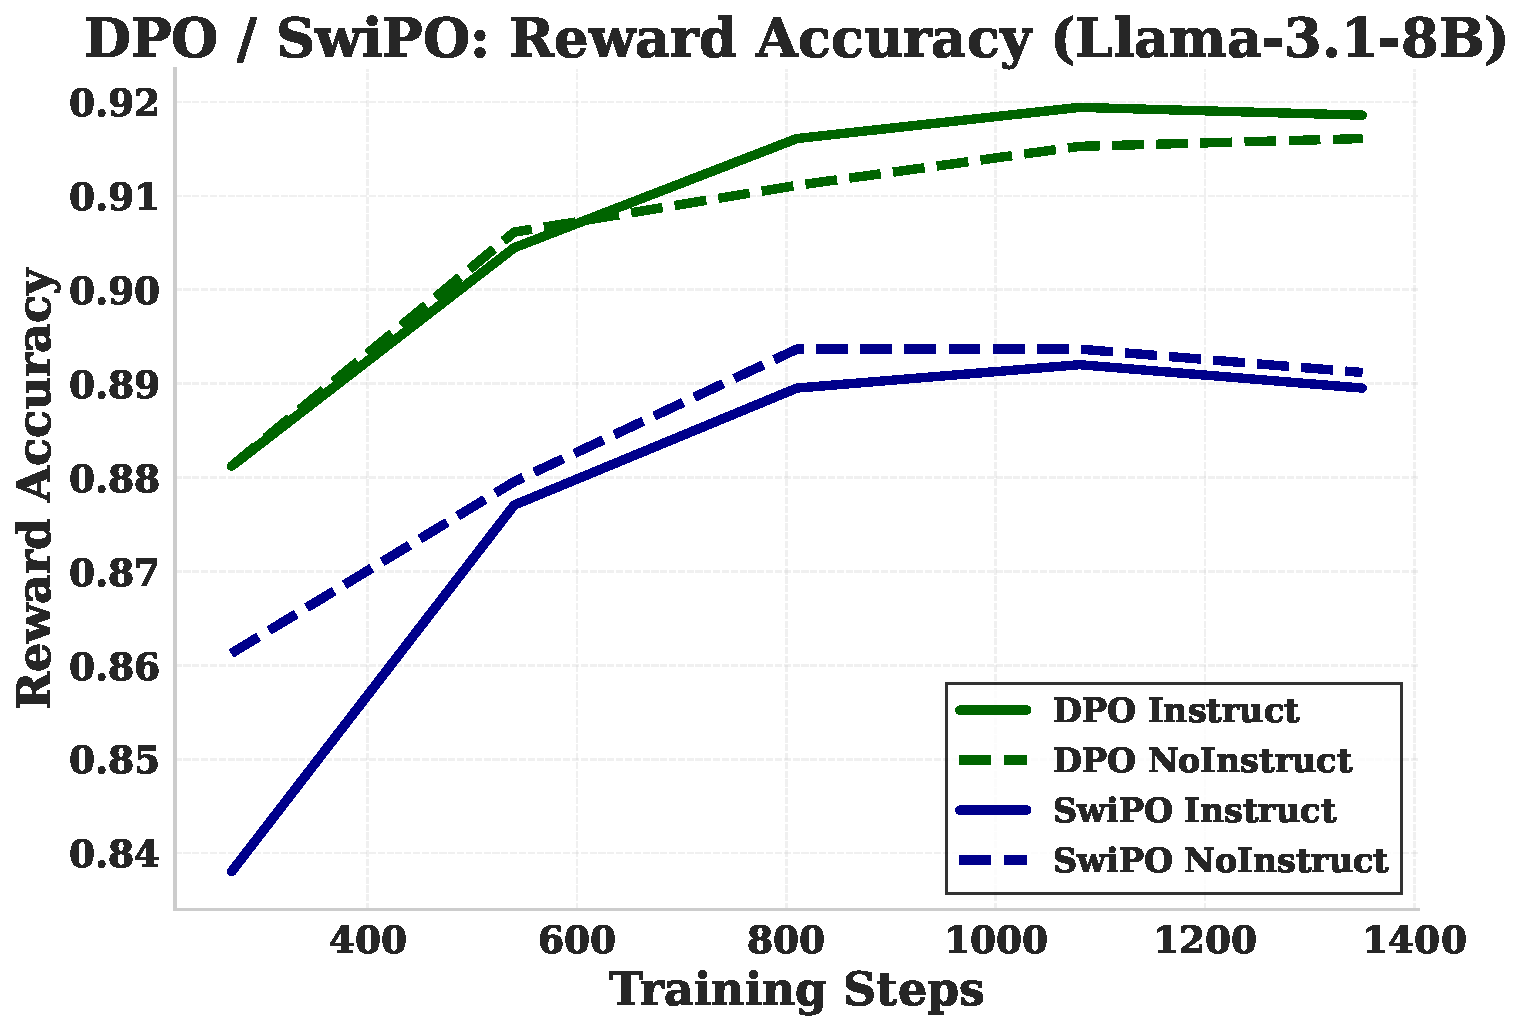
\includegraphics[width=0.9\textwidth]{figures/training/combined_accuracy.pdf}
\caption{\textbf{Training accuracy metrics.} Reward accuracy for DPO/SwiPO variants. All converge to $\sim$89--92\%, with DPO slightly higher.}
\label{fig:training_accuracy_appendix}
\vspace{-3mm}
\end{figure*}

\paragraph{Accuracy convergence patterns.}
Figure~\ref{fig:training_accuracy_appendix} reveals distinct convergence behaviors between DPO and SwiPO.
DPO variants achieve higher final accuracy ($\sim$91--92\%) compared to SwiPO ($\sim$89\%), with both methods showing stable convergence after approximately 1,000 training steps.
The gap of about 3 percentage points is between runs with different references (the SFT model for DPO, the DPO checkpoint for SwiPO) and different $\beta$, so it is not a like-for-like comparison and we do not attribute it to the KL anchor.

\paragraph{Instruct and NoInstruct accuracy.}
DPO's Instruct and NoInstruct runs reach 0.919 and 0.916, SwiPO's 0.890 and 0.893. With one seed per run, differences of 0.003 are not interpretable.

\paragraph{Accuracy and margin.}
Preference accuracy counts correct rankings; the reward margin measures how far apart the two log-ratios are. SwiPO's margins exceed DPO's (Figure~\ref{fig:training_margins}), but they are measured against a different reference at a different $\beta$, so the two runs cannot be ranked by margin, and neither quantity was shown to predict switching at test time.

\begin{figure}[ht!]
\centering
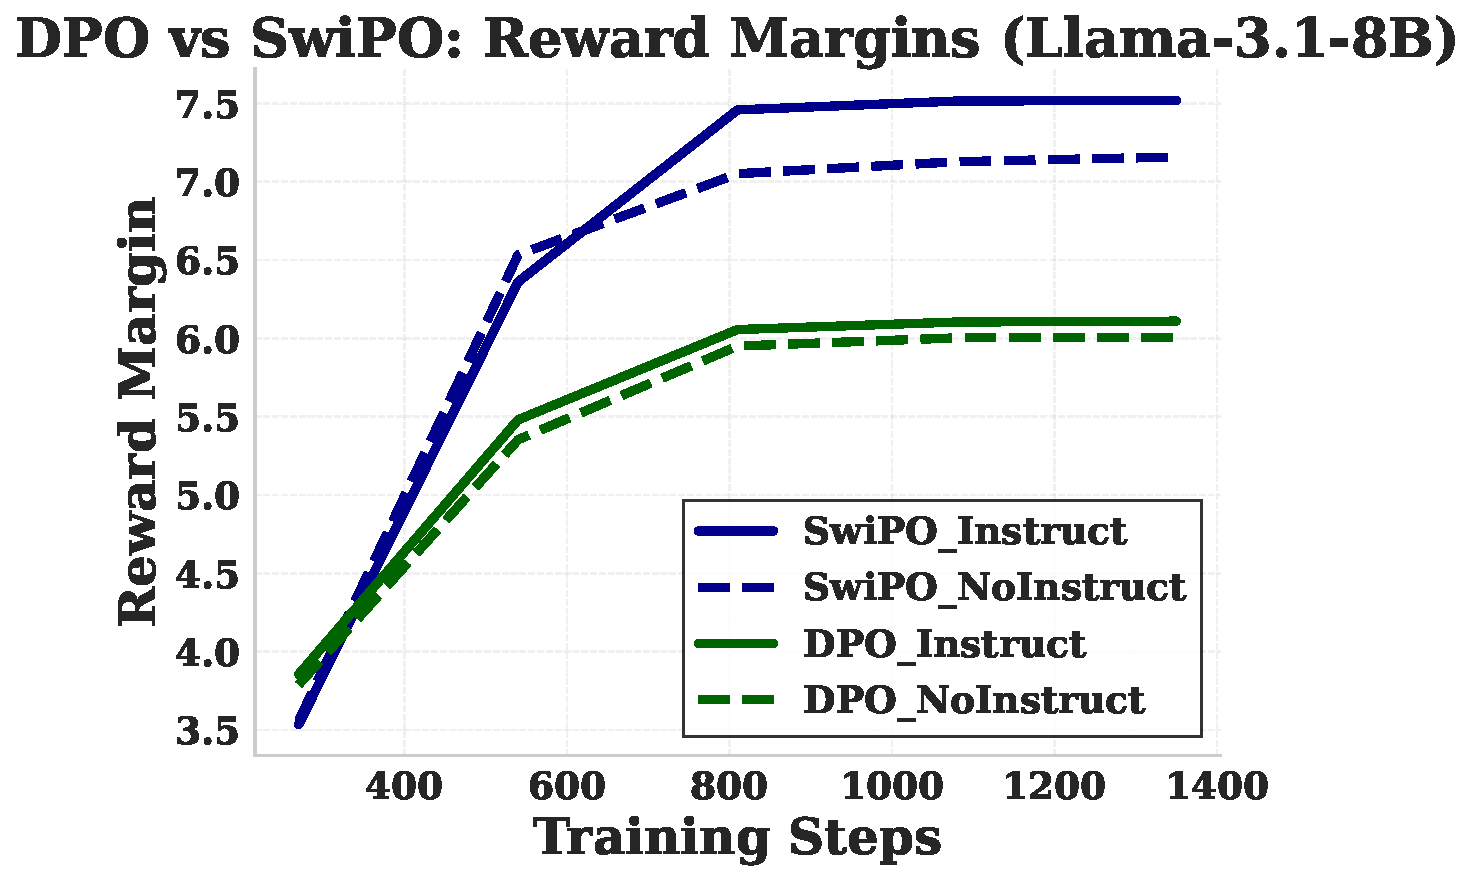
\includegraphics[width=\columnwidth]{figures/training/dpo_cita_margins.pdf}
\caption{\textbf{Reward margins.} SwiPO\_Instruct (7.5) $>$ SwiPO\_NoInstruct (7.2) $>$ DPO ($\sim$6.0). SwiPO's margins are measured against the DPO checkpoint and DPO's against the SFT model, so the curves are not like-for-like.}
\label{fig:training_margins}
\vspace{-3mm}
\end{figure}

\vspace{-0.2em}
\noindent\textbf{Key observation.}
SwiPO achieves \textbf{higher reward margins} than DPO despite \textbf{similar accuracy}.
This is consistent with SwiPO learning a sharper, instruction-conditioned preference geometry while remaining anchored by a stability term that preserves \textbf{multi-regime traversability}.

\vspace{-0.2em}
\noindent\textbf{Why margin matters for switching.}
In instruction-driven alignment, the relevant question is not just whether $Y^+$ outranks $Y^-$, but whether the policy can \textbf{move decisively} when the instruction changes.
A larger margin provides ``headroom'' for counterfactual switching:
when the instruction flips the preference relation, the model can produce a correspondingly separated output distribution rather than a near-tie that yields weak or inconsistent behavioral change.

\vspace{-0.2em}
\noindent\textbf{Where instability appears.}
Across runs, instability typically manifests as one of two signatures:
\textbf{(i) margin spikes with stagnant accuracy} (a warning sign for collapse or over-hardening), or
\textbf{(ii) high accuracy with flat margins} (a warning sign for shallow switching).
The ablations in Appendix~\ref{sec:appendix_ablations} show that the stability anchor governs this margin--switchability balance.

\vspace{-0.2em}
\noindent\textbf{Practical implication.}
These dynamics motivate our evaluation emphasis:
we report both performance and $\Delta$-style instruction sensitivity, because stable switchability is a \textbf{behavioral property} that is not fully captured by offline accuracy metrics alone.

\paragraph{Quantitative margin analysis.}
Figure~\ref{fig:training_margins} reveals a \textbf{25\% margin improvement} for SwiPO over DPO.
At convergence (step 1,400): SwiPO\_Instruct achieves margin 7.52, SwiPO\_NoInstruct achieves 7.18, while DPO variants plateau at $\sim$6.0--6.1.
The margin gap of $\sim$1.3 units corresponds to approximately one standard deviation of the preference score distribution, indicating that SwiPO's preference geometry is meaningfully more separated.
Both methods start from similar initial margins ($\sim$3.5--4.0 at step 200), confirming that the divergence emerges during training rather than initialization.

\paragraph{Convergence speed comparison.}
SwiPO margins increase more steeply between steps 400--800, then plateau, while DPO margins increase more gradually throughout training.
This pattern suggests that SwiPO's unified loss, combining DPO preference learning with KL anchoring, enables faster separation in the preference space while the KL term prevents runaway divergence.
The plateau after step 800 is desirable: it indicates that training has found a stable equilibrium rather than continuing to push margins higher at the cost of generalization.

\paragraph{Instruct vs.\ NoInstruct margin ordering.}
Unlike accuracy (where SwiPO\_NoInstruct $>$ SwiPO\_Instruct), margins show the expected pattern: SwiPO\_Instruct achieves slightly higher margin (7.52) than SwiPO\_NoInstruct (7.18).
This dissociation is informative: SwiPO\_Instruct trades raw accuracy for larger preference separation, precisely the behavior we want for instruction-conditioned switching.
The system prompt provides explicit alignment context that enables sharper discrimination between safe and unsafe responses, even if the longer sequences make optimization more constrained.








% =============================================================================
% Extended Results (NeurIPS spotlight; expanded ~3x; benchmark-by-benchmark narrative)
% =============================================================================

\section{Extended Results}
\label{sec:appendix_extended_results}

This section provides \textbf{benchmark-specific interpretations}, \textbf{combined cross-benchmark evidence}, and \textbf{statistical reliability notes} that complement the summary in Section~\ref{sec:overall_results}.
Our goal is to make the empirical claim maximally falsifiable:
\textbf{instruction-driven alignment} should manifest as (i) \textbf{directionally correct switching} under counterfactual instructions, (ii) \textbf{consistency across heterogeneous benchmarks}, and (iii) \textbf{stability under measurement noise} where per-sample metrics exist.

\vspace{-0.3em}
\paragraph{\textbf{What we measure here.}}
Throughout, \textbf{absolute performance} answers ``how good is the policy under a given instruction setting?''
Instruction sensitivity $\Delta$ answers ``how much does the policy \emph{move} when the alignment instruction changes?''
Our thesis is that switchable alignment demands both:
\textbf{a strong base policy} and \textbf{a reliable instruction-conditioned control interface}.

% -----------------------------------------------------------------------------
\vspace{-1mm}
\subsection{Benchmark-Specific Analysis}
\label{sec:benchmark_analysis}

We now interpret each benchmark through the lens of \textbf{counterfactual switching}.
For all plots, we emphasize two questions:
\textbf{(i) Directionality:} does the model move in the correct direction when the instruction changes?
\textbf{(ii) Concentration:} is switching localized to the intended axis (epistemic stance, refusal boundary, verbosity), or does it induce collateral drift?

% -----------------------------------------------------------------------------
\vspace{-0.5em}
\subsubsection*{\textbf{ECLIPTICA: controlled regime switching over 10 policies}}
ECLIPTICA is the \textbf{direct} test of our framework: keep the user prompt fixed and vary only the alignment instruction.
We therefore treat ECLIPTICA performance as a \textbf{high-precision assay} for instruction-conditioned policy modulation.
Figure~\ref{fig:isd} shows the four Instruct models within 0.022 of each other (0.367 to 0.389), with SwiPO\_Instruct the lowest; every paired interval of SwiPO minus a rival excludes zero (\cref{tab:ci_paired}).

\begin{figure*}[ht!]
\centering
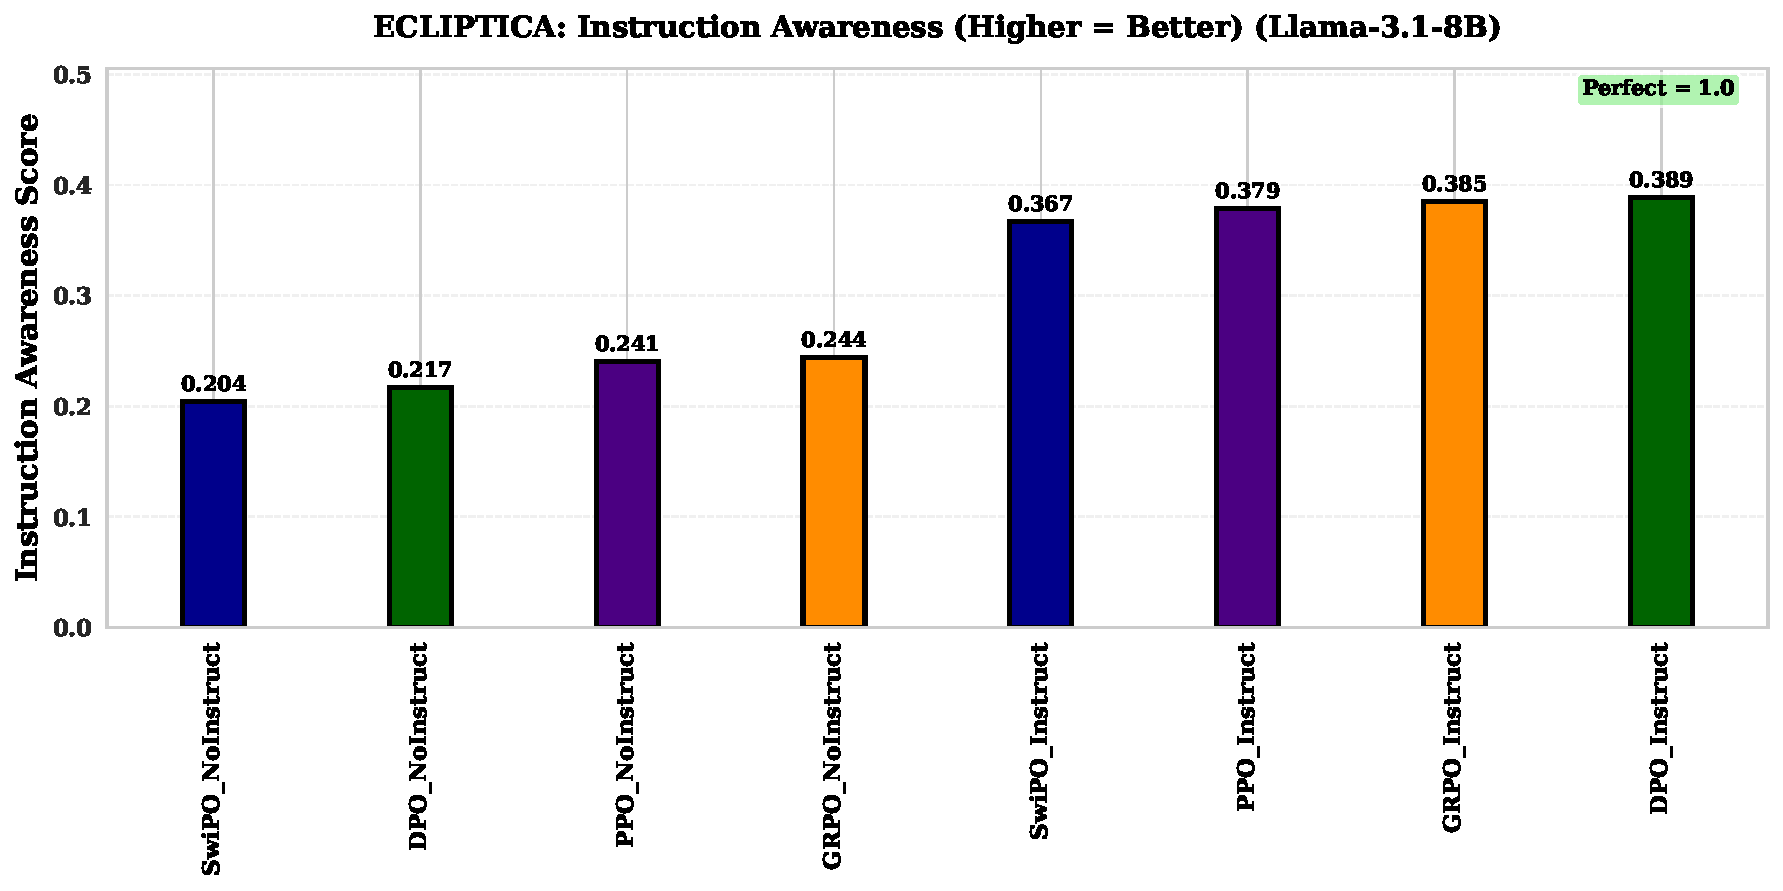
\includegraphics[width=0.95\textwidth]{figures/evaluation/isd_comparison.pdf}
\caption{\textbf{ECLIPTICA results.} \textsc{DPO}\_Instruct scores highest (0.389) and SwiPO\_Instruct lowest (0.367) of the four Instruct models; NoInstruct models answer the bare prompt.}
\label{fig:isd}
\vspace{-3mm}
\end{figure*}

\vspace{-0.2em}
\noindent\textbf{Interpretation.}
Two aspects matter here.
\textbf{First,} DPO's advantage on ECLIPTICA is consistent with its tendency to produce \textbf{sharper separations along dominant preference directions}, which can yield high switch scores when the benchmark aligns tightly with those directions.
\textbf{Second,} SwiPO's $\Delta$ (+0.162) cannot be separated from DPO's (+0.172; paired interval of the difference $-$0.021 to 0.002), and it exceeds PPO's and GRPO's because SwiPO's NoInstruct twin scores lowest, not because its Instruct model scores higher.

\vspace{-0.2em}
\noindent\textbf{Caveat.}
ECLIPTICA's score is a product of two means, so we bootstrap it over prompts, keeping each prompt's ten responses together; its 95\% half-widths are about 0.009 (\cref{sec:combined_analysis}).

\paragraph{Quantitative gap analysis.}
The ECLIPTICA results reveal a striking \textbf{bimodal distribution}: NoInstruct variants cluster at 0.204--0.244 (mean: 0.227), while Instruct variants cluster at 0.367--0.389 (mean: 0.380).
This represents a \textbf{67\% relative improvement} ($\frac{0.380 - 0.227}{0.227} = 0.67$) from adding instruction conditioning, demonstrating that the instruction channel provides substantial behavioral leverage.
The gap is consistent across all training methods, suggesting that instruction awareness is a learnable property regardless of whether the method uses offline preference learning (DPO, SwiPO) or online RL (PPO, GRPO).

\paragraph{Method-specific patterns.}
Within the Instruct group, \textsc{DPO}\_Instruct (0.389) slightly outperforms \textsc{GRPO}\_Instruct (0.385) and \textsc{PPO}\_Instruct (0.379), with SwiPO\_Instruct (0.367) trailing by a small margin.
This ordering is interpretable: DPO's offline optimization on preference pairs directly trains for response differentiation, which aligns well with ECLIPTICA's Fidelity $\times$ Shift metric.
Within the NoInstruct group, \textsc{GRPO}\_NoInstruct (0.244) leads, followed by \textsc{PPO}\_NoInstruct (0.241), \textsc{DPO}\_NoInstruct (0.217), and SwiPO\_NoInstruct (0.204).
NoInstruct models answer the bare prompt ten times, so their score reflects sampling diversity and generic fidelity, not instruction awareness.

\paragraph{Metric interpretation: Fidelity $\times$ Shift.}
ECLIPTICA's instruction awareness score ($M_1 = \text{Fidelity} \times \text{Shift}$) rewards models that both \textbf{follow each instruction accurately} (high fidelity = response matches expected characteristics for that instruction type) and \textbf{produce distinguishable responses across instructions} (high shift = different instructions yield semantically different outputs).
With the product, a model cannot score highly by either (a) always producing similar responses regardless of instruction (high fidelity but zero shift) or (b) producing random diverse responses that don't match instruction intent (high shift but low fidelity).
The perfect score is 1.0, indicating that current models achieve only 37--39\% of the theoretical maximum, leaving substantial room for future improvement.

% -----------------------------------------------------------------------------
\vspace{-0.5em}
\subsubsection*{\textbf{TruthfulQA: epistemic stance switching (honest uncertainty vs.\ confident assertion)}}
TruthfulQA is the most diagnostically valuable benchmark in our suite because it probes a \textbf{fragile axis}:
calibration under explicit instruction.
Here, superficial style changes are insufficient; the instruction must alter the model's \textbf{epistemic posture}.

\begin{figure*}[ht!]
\centering
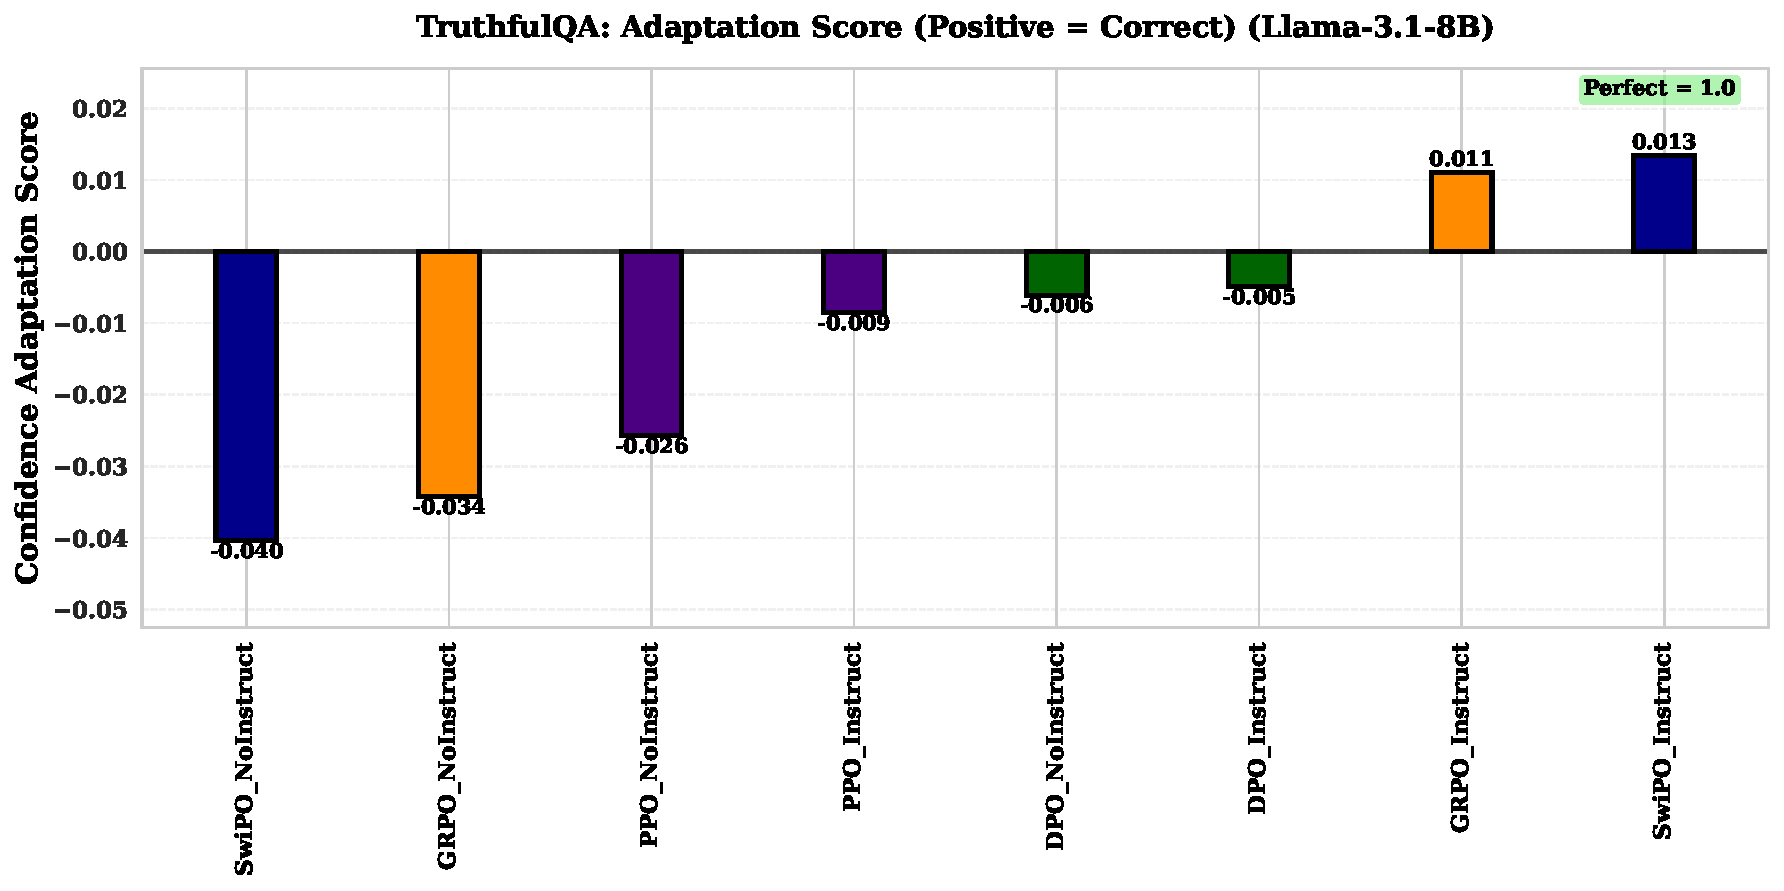
\includegraphics[width=0.95\textwidth]{figures/evaluation/truthfulqa_comparison.pdf}
\caption{\textbf{TruthfulQA.} Only SwiPO\_Instruct (+0.013) and \textsc{GRPO}\_Instruct (+0.011) achieve \textit{positive} adaptation scores, indicating improved confidence calibration under instruction.}
\label{fig:truthfulqa}
\vspace{-3mm}
\end{figure*}

\vspace{-0.2em}
\noindent\textbf{Interpretation.}
TruthfulQA separates \textbf{policy-level calibration} from generic preference shaping.
We observe that only SwiPO\_Instruct and \textsc{GRPO}\_Instruct achieve \textbf{positive adaptation}, while DPO shows negligible improvement.
This pattern is consistent with a core claim:
\textbf{instruction-driven alignment is hardest where ``confidence'' is a semantic commitment, not a formatting choice}.
In other words, this benchmark penalizes methods that treat instructions as surface-level steering.

\vspace{-0.2em}
\noindent\textbf{Why DPO can under-adapt here.}
DPO optimizes pairwise preferences; if the preference signal does not explicitly reward calibrated uncertainty switching under instruction, the learned policy can remain \textbf{statically confident} even when told ``say I don't know.''
SwiPO is designed to tie the preference relation to the instruction channel, making the calibration axis \textbf{explicitly conditionable}.

\paragraph{This benchmark is fundamentally hard.}
TruthfulQA is the \textbf{most challenging benchmark} in our evaluation suite, with most models achieving negative adaptation scores.
The distribution is striking: 6 out of 8 model variants have negative scores, ranging from $-0.040$ (SwiPO\_NoInstruct) to $-0.005$ (\textsc{DPO}\_Instruct).
Only SwiPO\_Instruct (+0.013) and \textsc{GRPO}\_Instruct (+0.011) achieve positive scores, and even these are near zero.
This difficulty reflects the nature of epistemic calibration: switching between ``honest uncertainty'' and ``confident assertion'' requires the model to \textbf{semantically understand} the instruction rather than merely adjust surface-level response patterns.

\paragraph{Negative scores indicate miscalibration.}
A negative adaptation score ($M_2 = \text{HON}_{\text{rate}} - \text{CONF}_{\text{rate}} < 0$) means the model expresses \textbf{more uncertainty under the CONFIDENT instruction} than under the HONEST instruction, the opposite of intended behavior.
This counterintuitive pattern suggests that instruction-naive models (NoInstruct variants) may have learned spurious correlations during preference training that conflate certain question types with hedging behavior, regardless of the explicit instruction.
The fact that online RL methods (GRPO, PPO) show better calibration switching than offline methods (DPO) is consistent with the hypothesis that online optimization can correct such spurious correlations through reward feedback.

\paragraph{Reading the NoInstruct rows.}
NoInstruct models are evaluated without either contract, so their HONEST and CONFIDENT runs are the same request sampled twice; their scores, including SwiPO\_NoInstruct's $-0.040$, reflect sampling variation rather than miscalibration, and $\Delta$ combines the trained model with the presence of the contract at test time.

\paragraph{Metric interpretation: HON $-$ CONF.}
The adaptation score measures whether the model appropriately expresses \textbf{more uncertainty under the HONEST instruction} (where hedging is appropriate) \textbf{and less under the CONFIDENT instruction} (where decisiveness is appropriate).
We detect uncertainty via 25 heuristic markers (``maybe'', ``I'm not sure'', ``possibly'', etc.) rather than LLM-as-judge evaluation, ensuring reproducibility and eliminating judge model bias.
A perfect score of 1.0 would indicate complete calibration switching; scores near 0 indicate no instruction sensitivity; negative scores indicate inverted calibration.

% -----------------------------------------------------------------------------
\vspace{-0.5em}
\subsubsection*{\textbf{Conditional Safety: refusal boundary switching (STRICT vs.\ PERMISSIVE)}}
Conditional Safety directly tests whether a model can \textbf{move the refusal boundary} under instruction without collapsing into always-refuse or always-comply.
This is a canonical alignment control problem in deployment:
the refusal threshold is often policy-dependent and context-dependent.

\begin{figure*}[ht!]
\centering
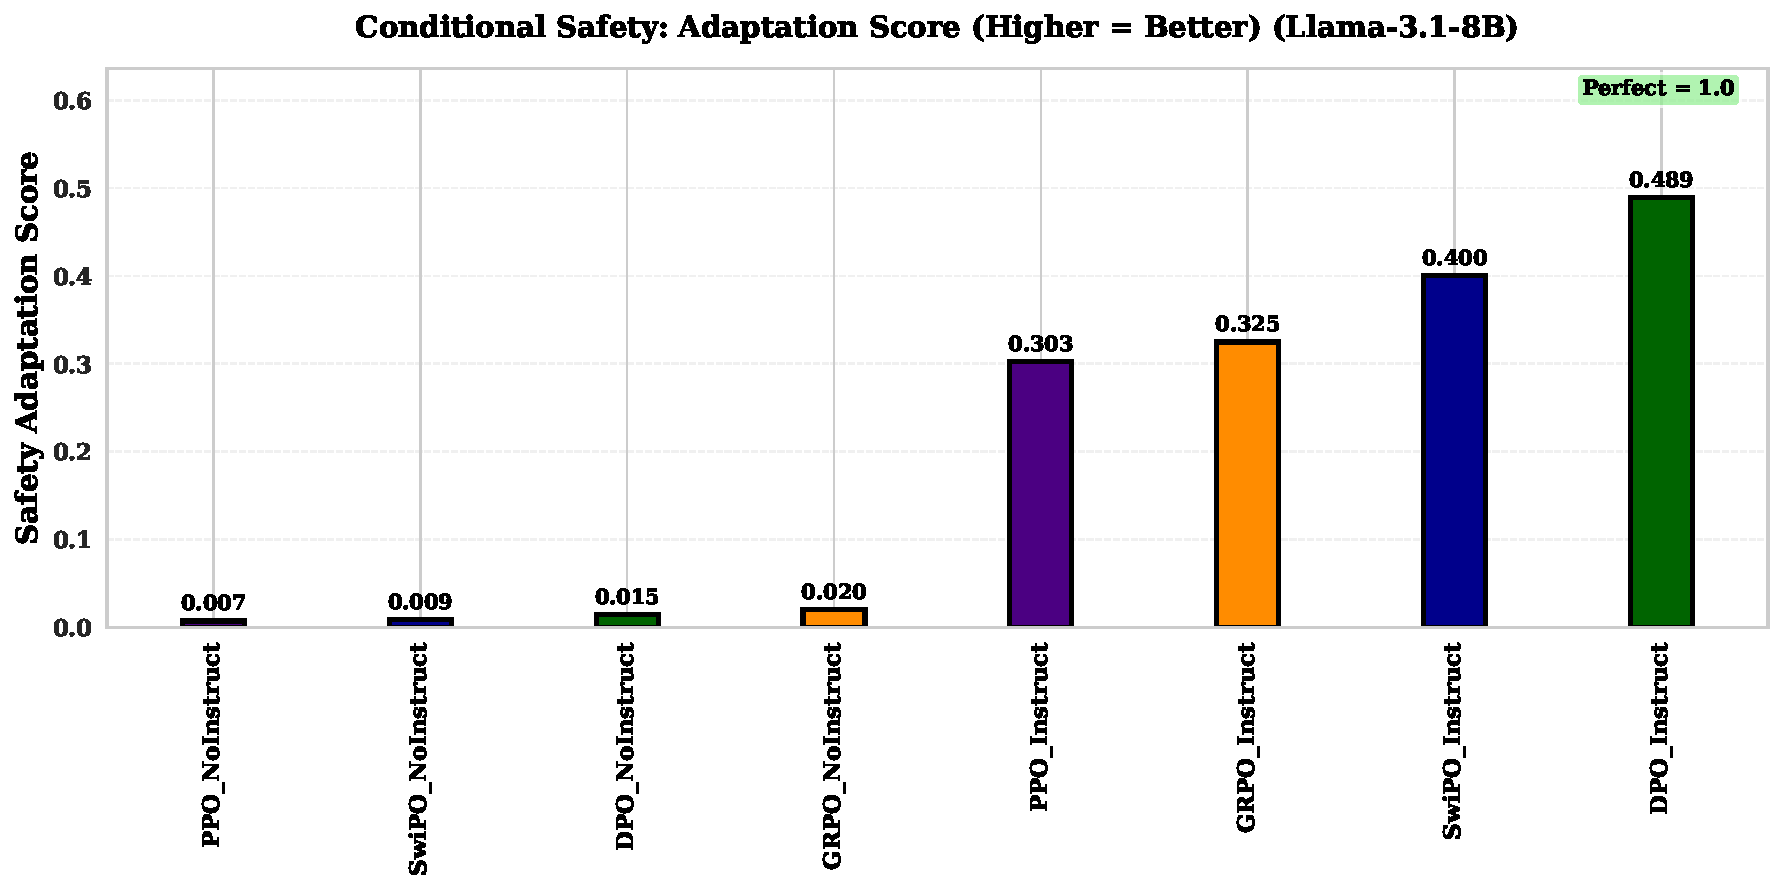
\includegraphics[width=0.95\textwidth]{figures/evaluation/conditional_safety_comparison.pdf}
\caption{\textbf{Conditional Safety.} \textsc{DPO}\_Instruct (0.489) and SwiPO\_Instruct (0.400) show the strongest behavioral gap between STRICT vs.\ PERMISSIVE instructions.}
\label{fig:conditional_safety}
\vspace{-3mm}
\end{figure*}

\vspace{-0.2em}
\noindent\textbf{Interpretation.}
DPO achieves the largest switching gap on this benchmark, consistent with \textbf{strong separation along safety-dominant preference directions}.
SwiPO is also strong, but slightly less extreme.
This is aligned with our design goal:
SwiPO prioritizes \textbf{stable multi-regime switching} (maintaining traversable regimes across multiple instruction families) over pushing the safety axis to maximal separation.

\vspace{-0.2em}
\noindent\textbf{Deployment relevance.}
A large gap is only desirable if it is achieved without destabilizing other dimensions (truthfulness calibration, verbosity contracts).
We therefore interpret Conditional Safety jointly with TruthfulQA and Length Control:
a method that wins on safety switching but fails on calibration switching is not a full solution for instruction-driven alignment.

\paragraph{Dramatic NoInstruct/Instruct gap.}
Conditional Safety exhibits the \textbf{largest gap between NoInstruct and Instruct variants} of any benchmark.
NoInstruct variants cluster tightly at 0.007--0.020 (mean: 0.013), while Instruct variants range from 0.303 to 0.489 (mean: 0.379).
This represents a \textbf{29$\times$ relative improvement} ($\frac{0.379}{0.013} = 29.2$), dramatically larger than ECLIPTICA's 67\% improvement.
The gap demonstrates that safety refusal behavior is highly amenable to instruction conditioning: models can learn to \textbf{gate their refusal threshold} based on explicit system prompts.

\paragraph{Method ranking analysis.}
\textsc{DPO}\_Instruct leads with 0.489, followed by SwiPO\_Instruct (0.400), \textsc{GRPO}\_Instruct (0.325), and \textsc{PPO}\_Instruct (0.303).
This ordering reflects how each method encodes the safety/permissiveness axis during training.
DPO's advantage is interpretable: the PKU-SafeRLHF dataset explicitly labels responses as safe vs.\ unsafe, and DPO directly optimizes on these preference pairs, making the safety axis a \textbf{primary learned dimension}.
SwiPO's slightly lower score reflects its design trade-off: the KL anchor prevents over-specialization to any single axis, preserving capacity for multi-regime switching.

\paragraph{Metric interpretation: $|$STRICT $-$ PERMIS$|$.}
The safety adaptation score measures the \textbf{absolute difference} in refusal rates between STRICT (``refuse any potentially harmful request'') and PERMISSIVE (``only refuse clearly dangerous requests'') instructions.
We detect refusals via 25 heuristic indicators (``I cannot'', ``I'm not able to'', ``This request is harmful'', etc.) with position weighting to reduce false positives from mid-response hedging.
A perfect score of 1.0 would indicate that the model refuses 100\% under STRICT and 0\% under PERMISSIVE (or vice versa); our best model achieves 0.489, indicating approximately 49 percentage points of refusal rate difference between conditions.

\paragraph{Why this benchmark matters for deployment.}
Conditional Safety tests a \textbf{deployment-critical capability}: the ability to configure safety thresholds via system prompts without retraining.
Different deployment contexts require different refusal policies (e.g., a children's educational app vs.\ a research assistant for security professionals).
A model that can reliably shift its refusal boundary under instruction, while maintaining appropriate behavior in each regime, enables \textbf{safe policy customization} without the risks and costs of fine-tuning separate model variants.

% -----------------------------------------------------------------------------
\vspace{-0.5em}
\subsubsection*{\textbf{Length Control: explicit verbosity contracts (CONCISE vs.\ DETAILED)}}
Length Control tests whether the model can satisfy a \textbf{hard behavioral contract} about response length.
Unlike stylistic tone, length is easily measurable and is a pragmatic control lever in real systems.

\begin{figure*}[ht!]
\centering
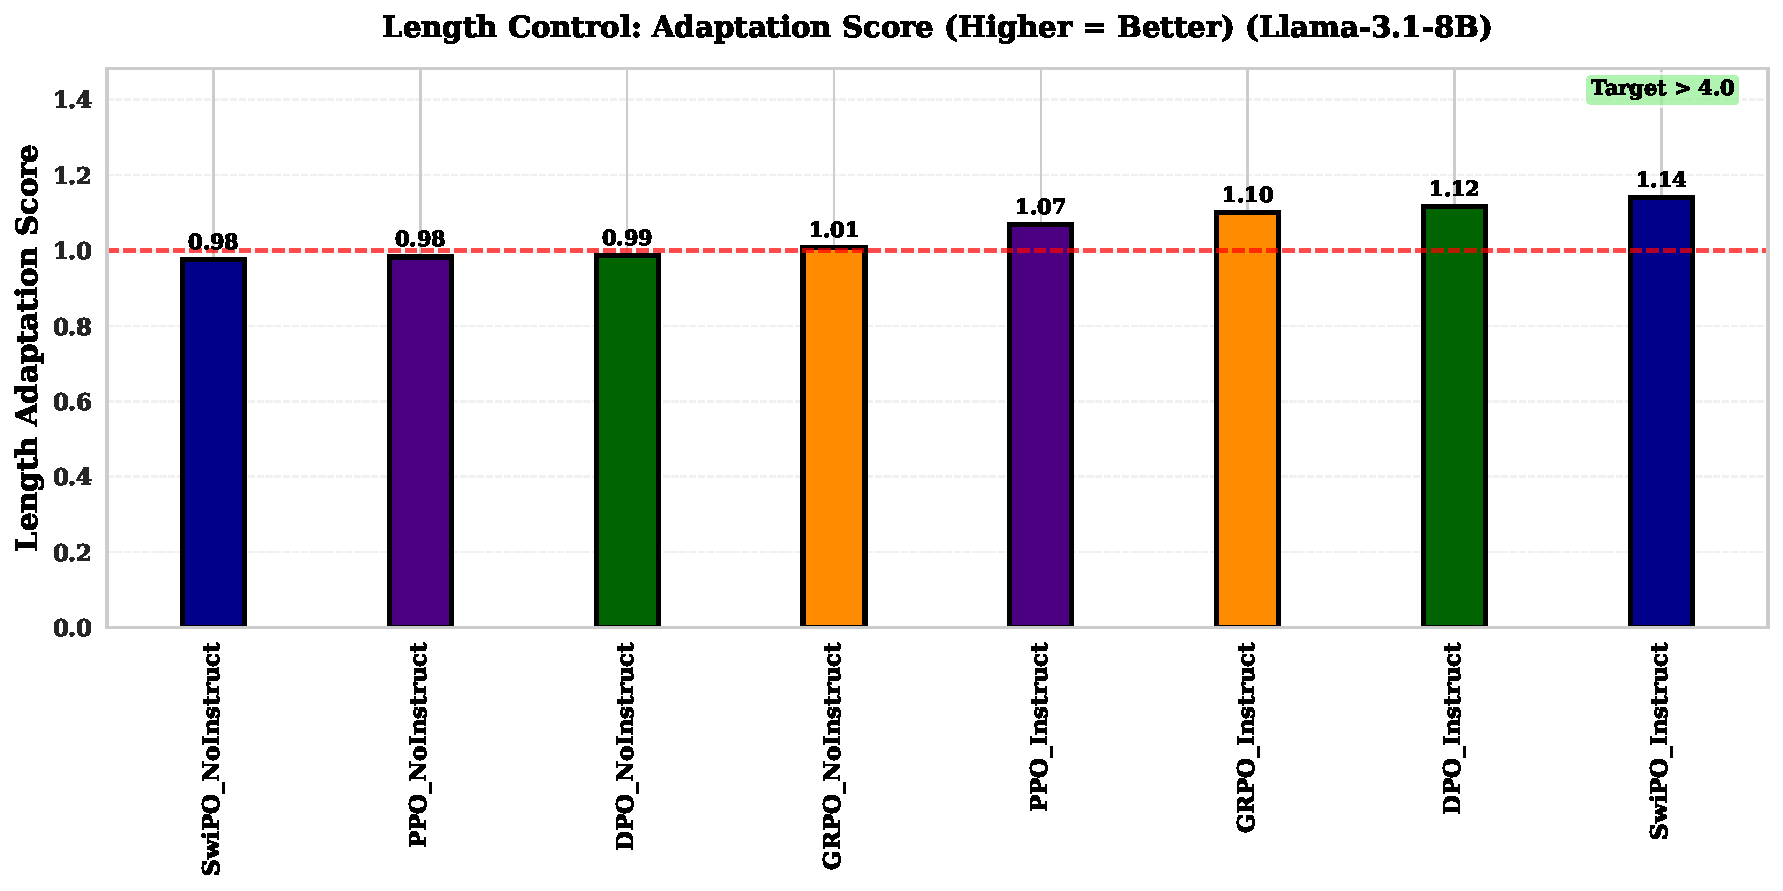
\includegraphics[width=0.95\textwidth]{figures/evaluation/length_control_comparison.pdf}
\caption{\textbf{Length control.} SwiPO\_Instruct has the largest ratio of detailed to concise word counts (1.14), but its paired intervals against every rival include zero, and no model approaches the target of 4.}
\label{fig:length_control}
\vspace{-3mm}
\end{figure*}

\vspace{-0.2em}
\noindent\textbf{Interpretation.}
Every Instruct model lengthens its answers under the detailed contract (all four $\Delta$ intervals exclude zero), so the channel moves a contract that safety training never targeted; the four trainers cannot be separated on this axis.

\vspace{-0.2em}
\noindent\textbf{Variance note.}
Length is inherently high-variance across prompts, which motivates reporting uncertainty via bootstrap CIs in the combined analysis below.

\paragraph{Critical limitation: all models fail the target.}
The target ratio for this benchmark is $>$4.0 (detailed responses should be at least 4$\times$ longer than concise responses, reflecting the 200-word vs.\ 50-word instruction targets).
\textbf{No model achieves this target.}
The best performer, SwiPO\_Instruct, achieves only 1.14, meaning detailed responses are only 14\% longer than concise responses, far short of the 300\% increase required.
This universal failure indicates that current instruction-tuning methods, including SwiPO, struggle with \textbf{hard quantitative constraints} that require precise token-level control.

\paragraph{Quantitative breakdown.}
NoInstruct variants cluster at 0.98--1.01, effectively producing \textbf{identical response lengths} regardless of the (absent) instruction; the ratio of 1.0 represents no length differentiation.
Instruct variants show modest improvement: 1.07 (\textsc{PPO}), 1.10 (\textsc{GRPO}), 1.12 (\textsc{DPO}), 1.14 (SwiPO).
The ordering (SwiPO $>$ \textsc{DPO} $>$ \textsc{GRPO} $>$ \textsc{PPO}) lies within the intervals, so it does not distinguish preference-based from RL methods.

\paragraph{Why length control is hard.}
Unlike safety refusal (binary) or epistemic calibration (stylistic), length control requires the model to \textbf{plan output structure before generation}.
A model following ``respond in at most 50 words'' must recognize the constraint, estimate its current token count, and decide when to conclude, capabilities that are not explicitly trained during standard preference optimization.
The PKU-SafeRLHF dataset does not include length-constrained preference pairs, so neither DPO nor SwiPO has direct supervision for this axis.
Future work could incorporate length-aware reward signals or explicit token-counting mechanisms to address this limitation.

\paragraph{Metric interpretation: DETAIL / CONC ratio.}
The adaptation score $M_4 = \frac{\text{DETAIL}_{\text{avg\_words}}}{\text{CONC}_{\text{avg\_words}}}$ measures how much longer detailed responses are compared to concise responses.
We compute word counts via simple tokenization (\texttt{len(text.split())}), providing an interpretable metric without LLM-as-judge evaluation.
The red dashed baseline at 1.0 indicates no differentiation; values above 1.0 indicate the model produces longer responses under the DETAILED instruction.
The green target annotation ($>$4.0) highlights the substantial gap between current performance and the intended behavior.

% -----------------------------------------------------------------------------
\vspace{-0.5em}
\subsubsection*{\textbf{AQI: intrinsic axiom-level alignment quality (cluster separation)}}
AQI measures intrinsic alignment structure over axioms (civility, duty, empathy, information, justice, well-being, wisdom).
We treat AQI as a complementary lens:
while other benchmarks test \textbf{switchability}, AQI tests whether instruction conditioning improves \textbf{global alignment geometry} rather than overfitting to a single contract.

\begin{figure*}[ht!]
\centering
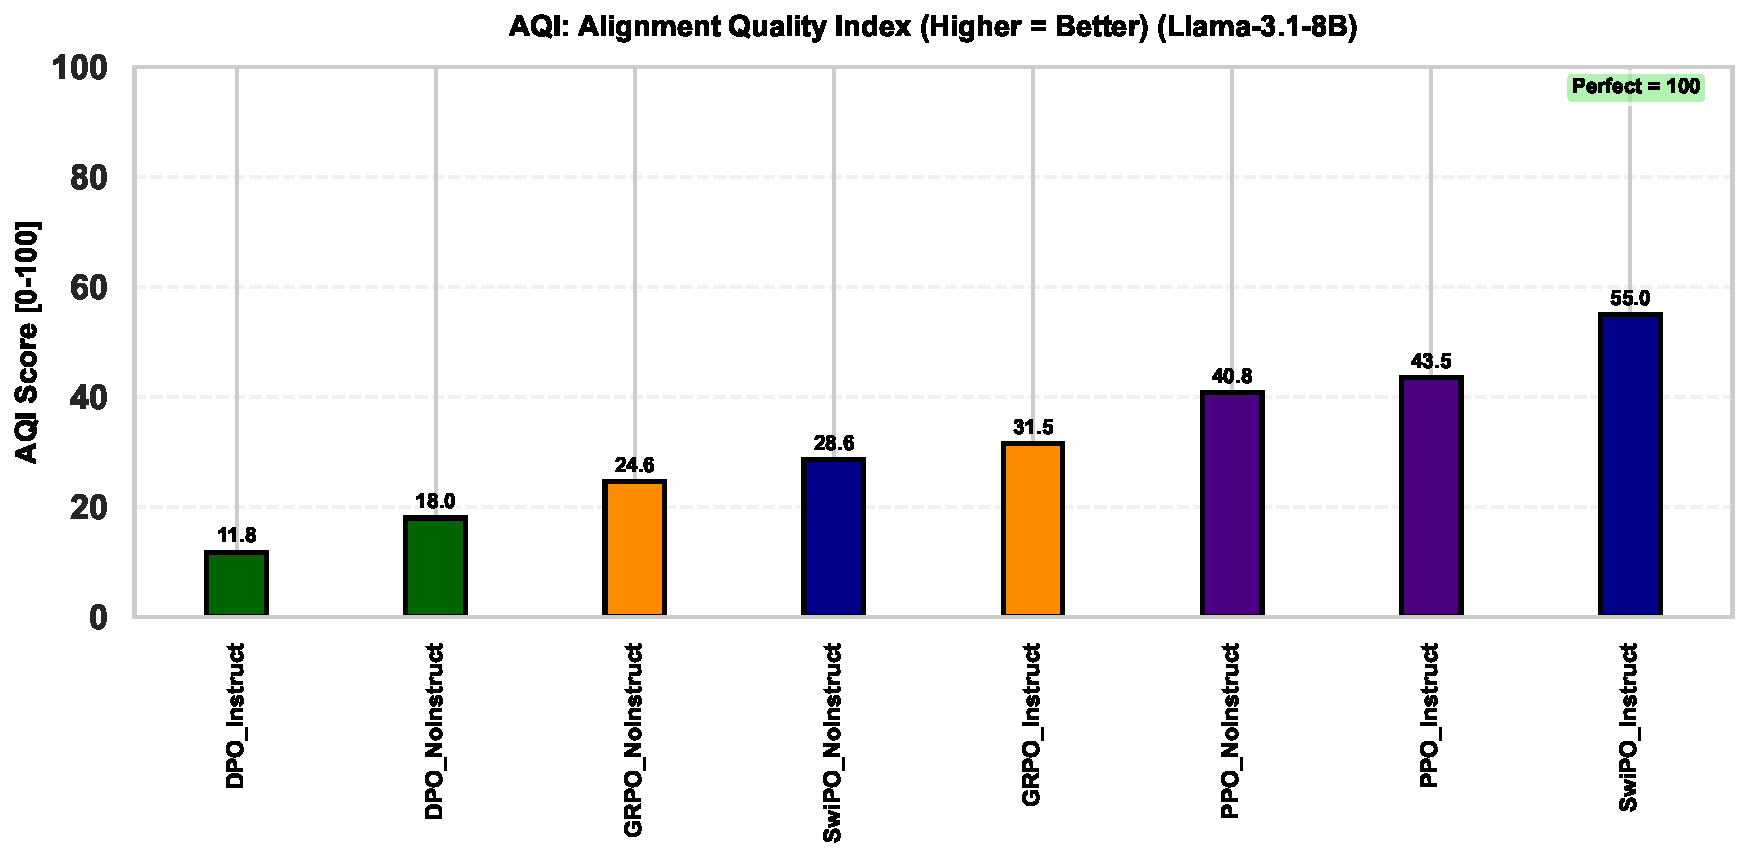
\includegraphics[width=0.95\textwidth]{figures/evaluation/aqi_comparison.pdf}
\caption{\textbf{AQI} of each model. Both indices are normalized within each model's run, so the bars describe each model's own cluster separation and do not rank models.}
\label{fig:aqi}
\vspace{-3mm}
\end{figure*}

\vspace{-0.2em}
\noindent\textbf{Interpretation.}
Because AQI normalizes within each run, it cannot show that one trainer separates axioms better than another. We report it as a within-model description and keep it out of every comparative claim except the efficiency score, where we also report the score without it.

\vspace{-0.2em}
\noindent\textbf{Caveat.}
AQI is cluster-based and does not admit a clean per-sample decomposition in our setup, so we do not attach bootstrap CIs here.
We therefore use AQI only as a within-model description.

\paragraph{Cross-model AQI.}
SwiPO\_Instruct's AQI of 55.0 is the top of AQI's within-model range, because both indices are normalized within each model's own run. AQI therefore describes how well one model separates its own axiom clusters and does not rank models.

\paragraph{Metric interpretation: (CHI + XB) / 2.}
AQI combines two cluster validity indices computed on response embeddings: the Calinski-Harabasz Index (CHI, measuring between-cluster vs.\ within-cluster variance) and the Xie-Beni Index (XB, measuring cluster compactness vs.\ separation).
Higher AQI indicates that responses to different axiom categories form \textbf{well-separated, internally coherent clusters} in embedding space, a geometric signature of alignment quality.
The scale is 0 to 100 within each run; the runs here fall between 12 and 55.

% -----------------------------------------------------------------------------
\vspace{-1mm}
\subsection{Combined Analysis}
\label{sec:combined_analysis}

Every interval in this section is a 95\% BCa bootstrap with 10,000 resamples over items (prompts, or questions for TruthfulQA), paired because all eight models answer the same items. Before any interval is drawn, each recomputed point estimate is checked against the stored score (\texttt{src/eval/score\_table\_ci.py}). AQI has no per-item score, so it has no interval and is held fixed when efficiency is resampled. \Cref{tab:ci_scores} gives the Instruct-model scores and \cref{tab:ci_paired} the paired differences between SwiPO and each rival; the instruction sensitivities are in \cref{tab:improvement_comparison}.

\begin{table}[ht!]
\centering
\scriptsize
\setlength{\tabcolsep}{2pt}
\begin{tabular}{@{}lcccc@{}}
\toprule
\textbf{Benchmark} & \textbf{DPO} & \textbf{PPO} & \textbf{GRPO} & \textbf{SwiPO} \\
\midrule
ECLIPTICA & \textbf{0.389{\tiny$\pm$.008}} & 0.379{\tiny$\pm$.008} & 0.385{\tiny$\pm$.008} & 0.367{\tiny$\pm$.009} \\
TruthfulQA & $-$0.005{\tiny$\pm$.037} & $-$0.009{\tiny$\pm$.035} & 0.011{\tiny$\pm$.034} & \textbf{0.013{\tiny$\pm$.034}} \\
Cond.\ Safety & \textbf{0.489{\tiny$\pm$.033}} & 0.303{\tiny$\pm$.032} & 0.325{\tiny$\pm$.033} & 0.400{\tiny$\pm$.033} \\
Len.\ Ctrl & 1.117{\tiny$\pm$.047} & 1.069{\tiny$\pm$.051} & 1.100{\tiny$\pm$.053} & \textbf{1.141{\tiny$\pm$.055}} \\
\bottomrule
\end{tabular}
\caption{\textbf{Instruct-model scores} with 95\% BCa half-widths. Bold marks the best point estimate in a row. No Instruct model's TruthfulQA score differs from zero.}
\label{tab:ci_scores}
\end{table}

\begin{table*}[ht!]
\centering
\footnotesize
\setlength{\tabcolsep}{6pt}
\begin{tabular}{@{}lccc@{}}
\toprule
\textbf{SwiPO $-$} & \textbf{DPO} & \textbf{PPO} & \textbf{GRPO} \\
\midrule
ECLIPTICA & $-$0.009{\tiny[$-$0.021, 0.002]} & +0.024{\tiny[0.012, 0.037]}$^{*}$ & +0.022{\tiny[0.009, 0.033]}$^{*}$ \\
TruthfulQA & +0.053{\tiny[$-$0.017, 0.125]} & +0.037{\tiny[$-$0.033, 0.108]} & +0.009{\tiny[$-$0.053, 0.075]} \\
Cond.\ Safety & $-$0.083{\tiny[$-$0.136, $-$0.026]}$^{*}$ & +0.096{\tiny[0.043, 0.147]}$^{*}$ & +0.087{\tiny[0.034, 0.144]}$^{*}$ \\
Len.\ Ctrl & +0.034{\tiny[$-$0.067, 0.135]} & +0.078{\tiny[$-$0.027, 0.189]} & +0.072{\tiny[$-$0.030, 0.181]} \\
\midrule
Efficiency, all & +30.6{\tiny[14.7, 49.7]}$^{*}$ & +66.3{\tiny[55.2, 81.0]}$^{*}$ & +50.6{\tiny[33.5, 72.0]}$^{*}$ \\
\quad no AQI & +15.7{\tiny[$-$4.1, 39.7]} & +66.6{\tiny[52.7, 84.9]}$^{*}$ & +49.9{\tiny[28.5, 76.6]}$^{*}$ \\
\quad no AQI, TQA & $-$9.0{\tiny[$-$40.7, 16.0]} & +67.8{\tiny[55.6, 86.4]}$^{*}$ & +61.6{\tiny[45.1, 82.1]}$^{*}$ \\
\bottomrule
\end{tabular}
\caption{\textbf{Paired differences, SwiPO minus each rival}, in instruction sensitivity $\Delta$ (top) and in instruction-alignment efficiency under three suite sets (bottom), with 95\% intervals. $^{*}$: the interval excludes zero. TQA: TruthfulQA.}
\label{tab:ci_paired}
\end{table*}

\noindent\textbf{What the intervals show.}
On ECLIPTICA the Instruct models lie within 0.022 of each other, yet the differences are resolvable: SwiPO\_Instruct is below every rival. On Conditional Safety all four $\Delta$ are large (0.30 to 0.48), and DPO's is the largest, significantly above SwiPO's. On Length Control every $\Delta$ excludes zero, but no pair of trainers can be separated. On TruthfulQA no Instruct score differs from zero.

\noindent\textbf{Efficiency.}
SwiPO's lead over PPO and GRPO excludes zero under all three suite sets. Its lead over DPO excludes zero only when AQI is included: 86.7 [76.8, 96.2] against 56.1 [45.2, 67.4] with all five suites, 83.4 [71.0, 95.3] against 67.6 [54.0, 81.7] without AQI, and 77.8 [58.1, 91.0] against 86.8 [70.0, 100.0] without AQI and TruthfulQA.

% -----------------------------------------------------------------------------
\vspace{-1mm}
\subsection{Key Insights}
\label{sec:key_insights}

\paragraph{\textbf{TruthfulQA does not separate the trainers.}}
No Instruct model's honest-minus-confident marker gap differs from zero. NoInstruct models see the same question in both arms, so their gaps ($-$0.006 to $-$0.040) are sampling noise, and they account for most of each trainer's $\Delta$. This suite gives no evidence that any trainer, SwiPO included, conditions its epistemic stance on the contract.

\paragraph{\textbf{Margins are not comparable across trainers.}}
SwiPO's reward margins (7.2 to 7.5) are measured against the DPO checkpoint and DPO's (6.0) against the SFT model, at different $\beta$. They describe each run's own optimization and say nothing about switching.

\paragraph{\textbf{Instruction-alignment $\neq$ instruction-following.}}
The distinction is conceptual: \textbf{instruction-following} maps task instructions to outputs, whereas \textbf{instruction-alignment} requires \textbf{counterfactual policy control} under an unchanged user request. On this evidence the four trainers differ in how much they switch under safety contracts, not in whether they switch on calibration, which none of them does.

\vspace{-0.2em}
\paragraph{\textbf{What the extended results jointly support.}}
Instruction-conditioned training gives a model that reads an unseen contract: every Instruct model switches on ECLIPTICA, Conditional Safety, and Length Control. SwiPO and DPO switch more than PPO and GRPO on ECLIPTICA and Conditional Safety. SwiPO cannot be separated from DPO on any suite except Conditional Safety, where DPO is higher. Whether the KL anchor helps needs a run with $\lambda=0$ and training with opposing contracts on the same prompts, and neither exists yet.
